\documentclass[onecolumn]{IEEEtran}
\textheight=24cm
\textwidth=18cm
\topmargin=-2cm
\oddsidemargin=0cm
\usepackage[utf8x]{inputenc}
\usepackage{graphicx}
\usepackage{times}
\usepackage[tbtags]{amsmath}
\usepackage{cite}
\usepackage[all]{xy}
\usepackage{subfigure}
\usepackage{wrapfig}
\usepackage{multicol}
\usepackage{url}
\usepackage[tbtags]{amsmath}
\usepackage{amsmath,amssymb,amsfonts,amsbsy}
\usepackage{bm}
\usepackage[all]{xy}
\usepackage[centerlast, small]{caption}
\usepackage[colorlinks=true, citecolor=blue, linkcolor=blue, urlcolor=blue, breaklinks=true]{hyperref}

\begin{document}
\title{Informe 2 de Matlab}
\author{David Ricardo Martínez Hernández Código: $261931$\\
	Juan David Ramos López Código: $261667$}
\maketitle
\markboth{Universidad Nacional de Colombia}{}{}
\section{Descripción del programa}
\noindent
Se genero la señal de entrada de la fig \ref{fig1}, se multiplico en tiempo con una señal $cos(2 \pi fx)$ donde:\\
$f$ es una frecuencia de $40 \ \ KHz$\\
$x$ es el vector o el intervalo de frecuencia que va desde $-1\ \ ms$ hasta $1\ \ ms$,\\
como se muestra en la fig \ref{fig2}.\\
Para que el programa funcionara la frecuencia de muestreo de la señal de  entrada  es mayor que la frecuencia del coseno para que se obtenga la señal deseada,
\begin{verbatim}
f=40000;%frecuencia del coseno
fm=41000;%frecuencia de muestreo
x=-1/1000:1/(2*pi*fm):1/1000;
\end{verbatim}
\noindent
si no se obtendrá un coseno con diferentes amplitudes, si se hace de esa manera no se obtendrá una correcta modulación y demodulación.\\
El parámetro $M$ se escogió de $1000$, debido a que la señal tiene como mínimo $80$ muestras en tiempo y tendrá un máximo de $360$.
\begin{figure}[h]
	\centering
		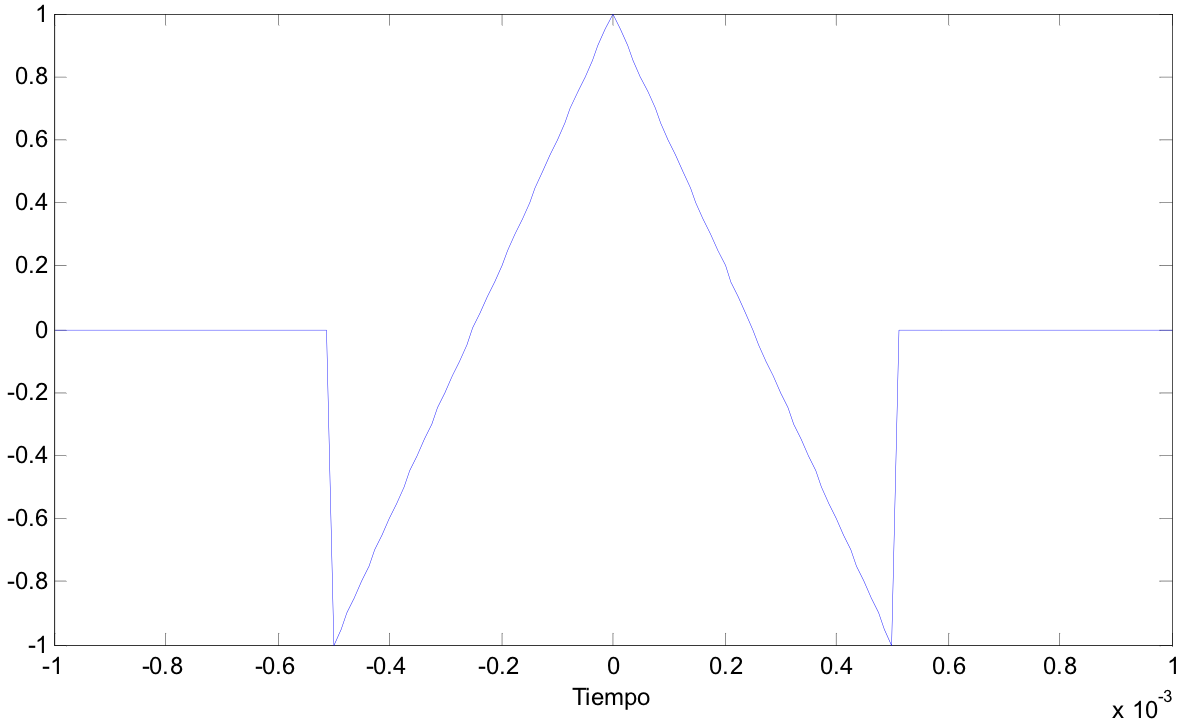
\includegraphics[scale=0.25]{0.png}
	\caption{Señal de entrada}
    \label{fig1}
\end{figure}

\begin{figure}[h]
	%\centering
		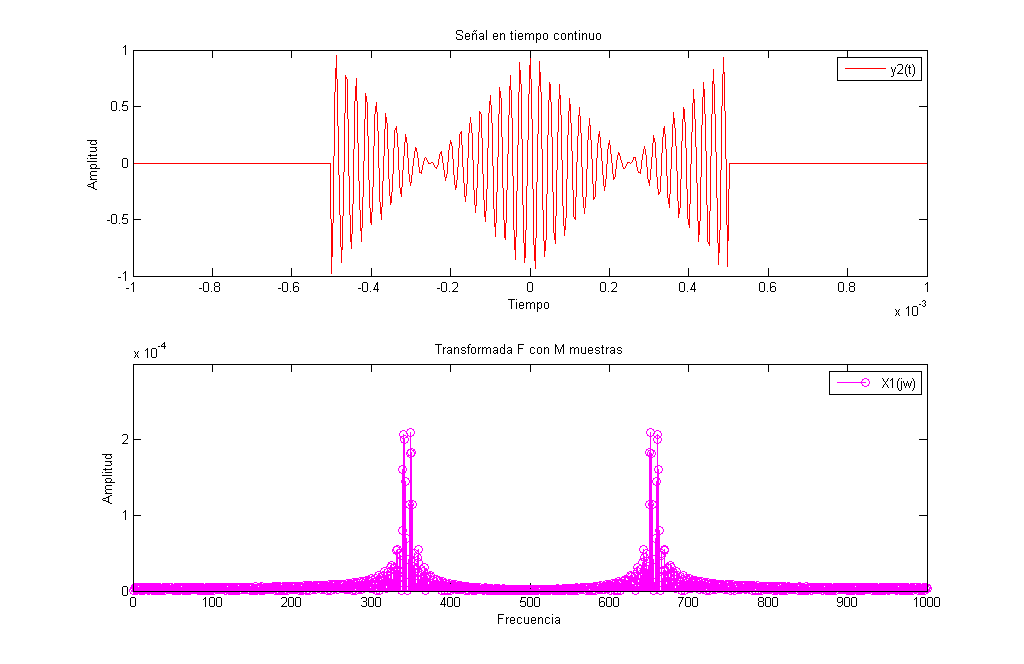
\includegraphics[scale=0.55]{1.png}
	\caption{Señal de entrada multiplicada por $cos(2\pi fx)$ en tiempo y en frecuencia}
    \label{fig2}
\end{figure}
\noindent
\begin{verbatim}
y=funcion(x);
y1=cos(2*pi*f*x);
y2=y.*y1;
YX2=fftshift((1/(2*pi*fm))*(fft(y2,M)));
\end{verbatim}
\noindent
donde\\
$y$ es la señal de entrada\\
$y_1$ es la señal coseno\\
$y_2$ es la multiplicación de $y$ com $y1$\\
$YX_2$ es la transformada de Fourier de la señal $y2$\\
Después se procedió a multiplicar nuevamente la señal de entrada figura \ref{fig1} con el coseno dando como resultado la figura \ref{fig3}
\begin{figure}[h]
	%\centering
		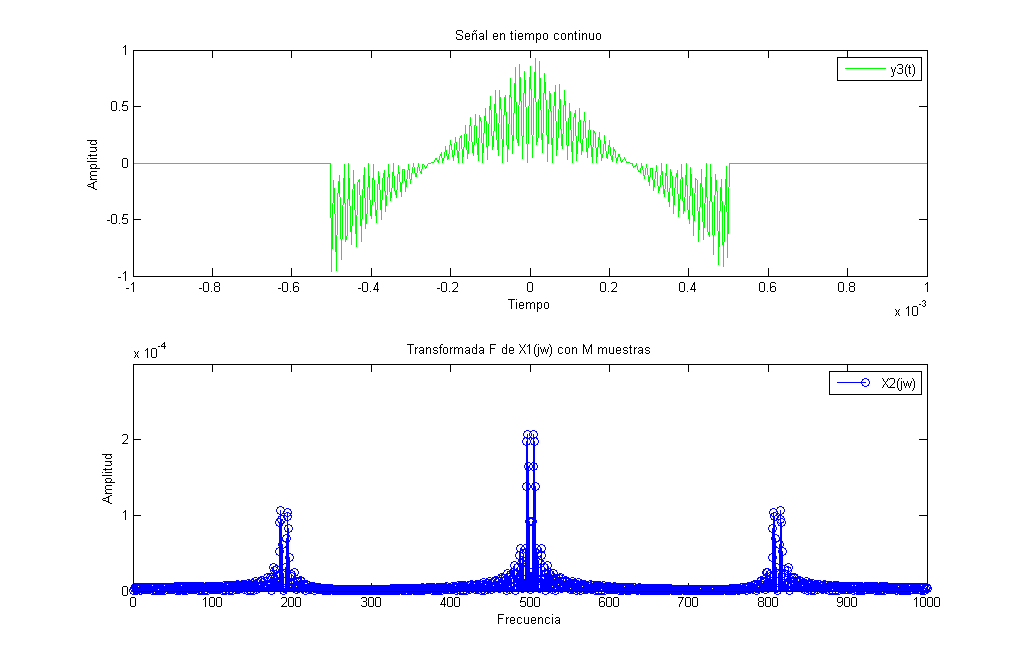
\includegraphics[scale=0.55]{2.png}
	\caption{Señal de entrada multiplicada por $cos^2(2\pi fx)$ en tiempo y en frecuencia}
    \label{fig3}
\end{figure}
\begin{verbatim}
y3=y.*y1.^2
YX3=fftshift(1/(2*pi*fm)*(fft(y3,M)))
\end{verbatim}
\noindent
donde\\
$y_3$ es la multiplicación de $y*y1^2$\\
$YX_3$ es la transformada de Fourier de la señal $y3$\\
\\
Como la transformada de $y1*cos^2(2\pi fx)$ tiene tres ``impulsos'' iguales pero con diferente magnitud y corridas en frecuencia se debe aplicar un filtro pasa-bajos para que solo se obtenga el ``impulso'' del medio, como se muestra en la figura \ref{fig4}
\begin{figure}[]
	%\centering
		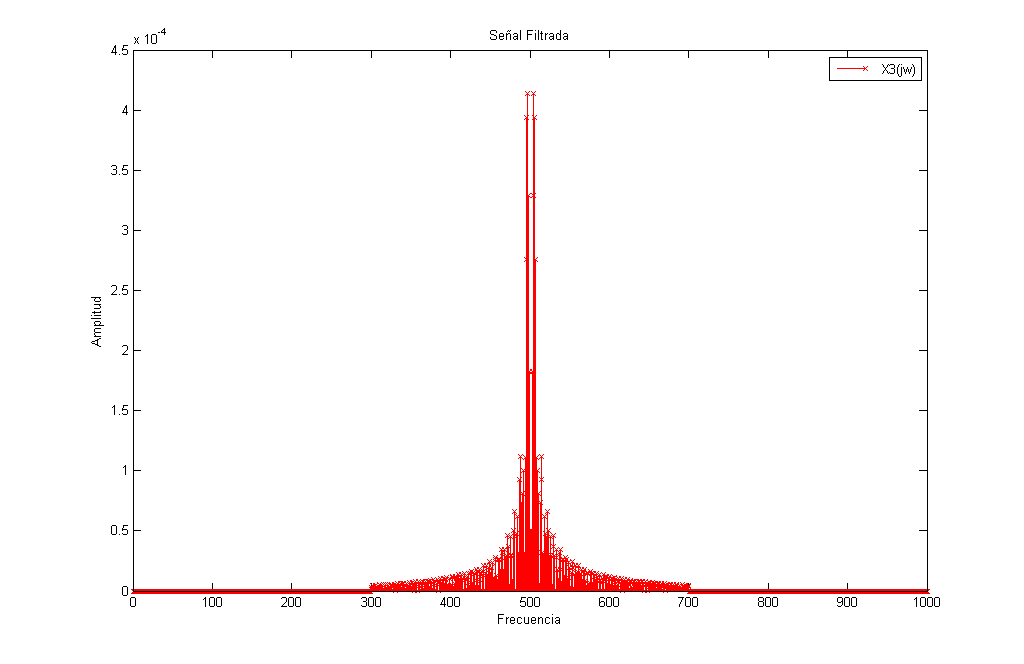
\includegraphics[scale=0.55]{3.png}
	\caption{Señal filtrada}
    \label{fig4}
\end{figure}
\begin{verbatim}
filtro=ones(1,M);
for i=1:M
	if (i<M/2-200 || i>M/2+200)
		filtro(i)=0;
	end
end
y5=2*filtro.*YX3;
\end{verbatim} 
\noindent
Para este filtro se utilizo una matriz de $1's$ para que al momento de ser filtrada con el \verb for \verb i=1:M  y con el\\ \verb if \verb (i<M/2-200 \verb || \verb i>M/2+200) quedara la señal original en el intervalo deseado, dando como resultado la fig \ref{fig4}, en el condicional el ancho del filtro puede ser modificado, para volverlo mas fino, cambiando el valor de $200$ por cualquier otro número.\\\\
La señal filtrada se encuentra en la figura \ref{fig5}

\begin{figure}[]
	%\centering
		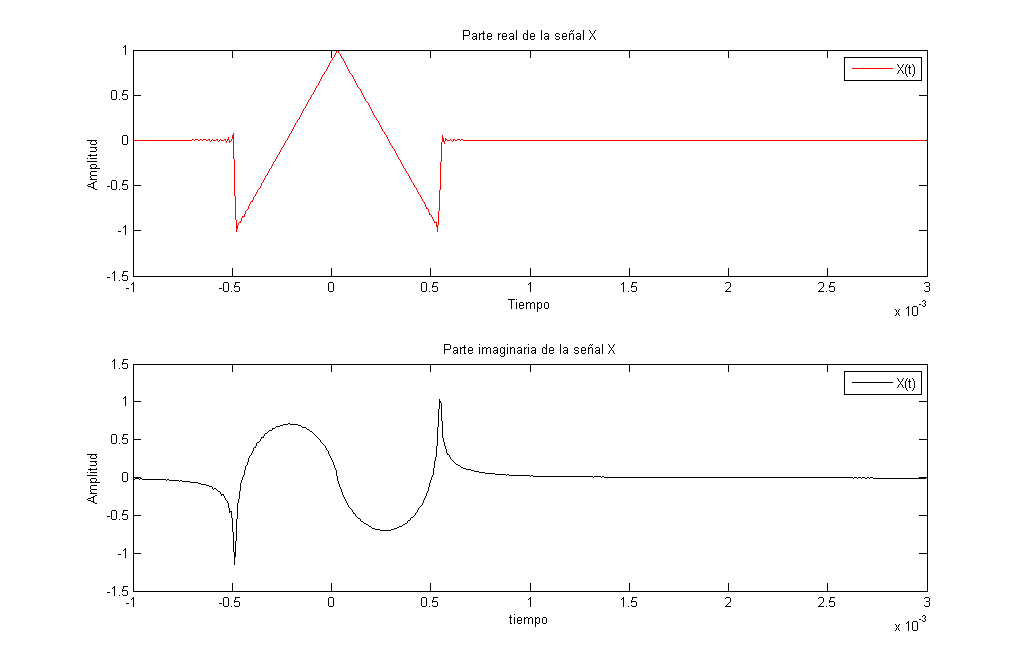
\includegraphics[scale=0.55]{4.png}
	\caption{Salida de la trasnformada inversa de la función $y5$, parte real y parte imaginaria}
    \label{fig5}
\end{figure}
\begin{verbatim}
X=ifft(y5,M/2)/(1/(2*pi*fm));%transformada inversa filtrada
xreal=-1/1000:2/(500*M/2-1):3/1000;
\end{verbatim}
\noindent
donde\\
$X$ es la Transformada inversa de la señal filtrada ($y5$)\\
$x_{real}$ es el vector para el ajuste de los índices de la trasnformada inversa\\\\
Los índices fueron calculados de la siguiente manera.
\begin{itemize}
 \item Como la ifft de $y_5$ tiene un total de $500$ muestras, la señal original se encuentra entre la muestra $1$ y la $250$, es decir en ese intervalo se encuentra la señal original.
 \item Como la señal de entrada tiene $516$ muestras en su totalidad, desde $-1 \ \ ms$ hasta $1\ \ ms$, la señal $y_5$ tiene un intervalo de tiempo desde $-1 \ \ ms$ hasta $3\ \ ms$, es decir 2 veces más de tiempo, pero la duración de la señal sigue siendo de $2\ \ ms$. Como el tiempo total es de $4\ \ ms$ y el tamaño total de la ifft es de $500$ muestras, se calculo con una regla de $3$ simple, es decir:
$$\frac{4*10^{-3}} {\frac{M}{2}-1}$$
\noindent
El denominador $\frac{M}{2}-1$ se le resta $1$ debido a que se debe tomar el total de la muestra menos $1$ para obtener el valor deseado.
\end{itemize}
\section{Conclusiones}
\begin{itemize}
 \item La frecuencia de muestreo debe ser mayor a la mayor de las frecuencias establecidas en el problema para que no hallan errores al momento de calcular las trasnformadas de Fourier.
 \item Para poder demodular la señal es necesario hacerlo con la mitad de las muestras para obtener la señal original.
 \item MatLab es una gran herramienta para ayudarnos a calcular la modulación y demodulación de señales y aproximarlas a modelos muy reales de una manera muy sencilla y eficaz.
\end{itemize}
\end{document}